\documentclass[10pt]{beamer}

\usetheme[progressbar=frametitle]{metropolis}
\usepackage{appendixnumberbeamer}
\usepackage{booktabs}
\usepackage[scale=2]{ccicons}
\usepackage{pgfplots}
\usepgfplotslibrary{dateplot}
\usepackage{graphicx}
\usepackage{xspace}
\newcommand{\themename}{\textbf{\textsc{metropolis}}\xspace}

\title{Interactr}
\subtitle{Iteration 2}
\date{\today}
\author{Jelle de Coninck, Hannes De Smet, Bruno Vandekerkhove, Shani Vanlerberghe}
\institute{KULeuven}
% \titlegraphic{\hfill\includegraphics[height=1.5cm]{logo.pdf}}

\begin{document}

\maketitle

\begin{frame}{Table of contents}
  \setbeamertemplate{section in toc}[sections numbered]
  \tableofcontents[hideallsubsections]
\end{frame}

\section{Design}

\begin{frame}[fragile]{Design - Typical Flow}
\begin{center}
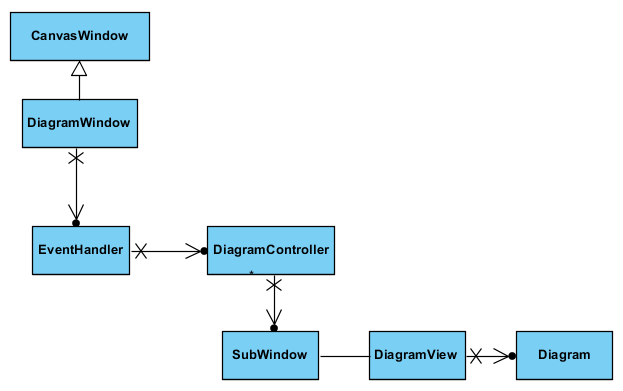
\includegraphics[width=1\textwidth]{flow}
\end{center}
\end{frame}

\begin{frame}[fragile]{Design - Domain Model (Mapping)}
\noindent\begin{minipage}{0.5\textwidth}% adapt widths of minipages to your needs
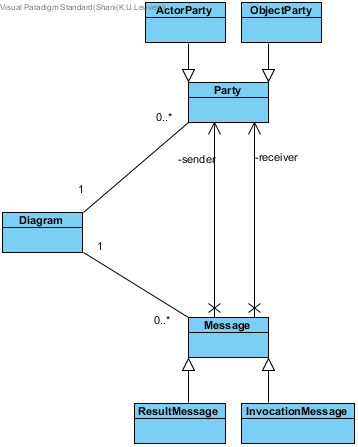
\includegraphics[width=1\textwidth]{domain}
\end{minipage}%
\hfill%
\begin{minipage}{0.5\textwidth}\raggedleft
\begin{itemize}
	\item Low representational gap
	\item Virtually nothing changed
	\item Prefixes fixed
	\end{itemize}
\end{minipage}
\end{frame}

\begin{frame}[fragile]{Design - DiagramController}
\begin{itemize}
\item Used to be quite central (managed \texttt{Diagram} itself)
\item Now only keeps track of subwindows
\item Each \texttt{DiagramView} manages the \texttt{Diagram} directly
\item Synchronisation done with Observer pattern (see later)
\end{itemize}
\begin{center}
\vspace{1cm}
\texttt{Controller - Low Coupling}
\end{center}
\end{frame}

\begin{frame}[fragile]{Design - Subwindows}
\texttt{DiagramController} uses sorted list of subwindows (drawn in reverse order)
\begin{itemize}
\item Class \texttt{SubWindow}
\item Subwindows and views draw themselves (i.e. drawing is delegated)
\item Use of clipping rectangle set on \texttt{PaintBoard}
\end{itemize}
\begin{center}
\vspace{1cm}
\texttt{Information Expert - Polymorphism}
\end{center}
\end{frame}

\begin{frame}[fragile]{Design - Synchronisation}
\begin{center}
\vspace{1cm}
\texttt{Pure Fabrication - Observer (GoF)}
\end{center}
\end{frame}

\begin{frame}[fragile]{Design - GoF Patterns}
4 patterns :
\begin{itemize}
\item \texttt{PaintBoard} : Facade
\item \texttt{proposedFigure()} : Factory Method
\item \texttt{DiagramNotificationCenter} : Singleton \& Observer
\end{itemize}
\end{frame}

\begin{frame}[fragile]{Design - Coding}
\begin{itemize}
\item Refactored here and there (eg. \texttt{Extract Method} in response to \texttt{Duplication})
\item Defensive programming - use of exceptions
\item Everything is documented (informally)
\end{itemize}
\end{frame}

\section{Extensibility}

\begin{frame}[fragile]{Extensibility - Observer}
3 methods considered :
\begin{itemize}
\item \texttt{DiagramObserver} interface with one method \texttt{diagramDidUpdate}, passing along the update type and associated parameters (in a dictionary)
\item Keeping \texttt{SubWindow} and \texttt{DiagramView} in separate lists as observers
\item \texttt{DiagramObserver} interface with methods with \texttt{default} implementations
\end{itemize}
Second method currently in use, last two methods similar in terms of extensibility. First method causes messy code with lots of \texttt{instanceof}.
\end{frame}

\section{Testing}

\begin{frame}[fragile]{Testing - Methods}
Combination of :
\begin{itemize}
\item Recordings
\item Step-by-step recordings
\item Unit tests
\end{itemize}
\end{frame}

\begin{frame}[fragile]{Testing - Coverage}
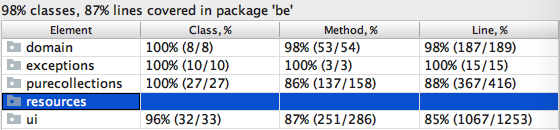
\includegraphics[width=1\textwidth]{coverage}
%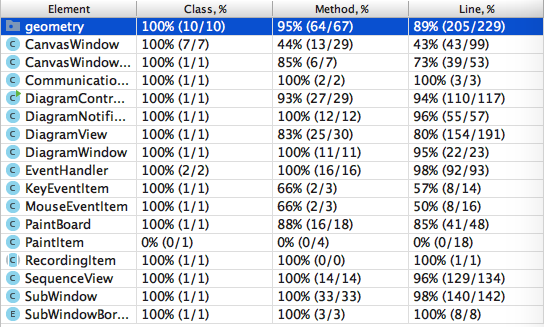
\includegraphics[width=1\textwidth]{coverage2}
\end{frame}

\section{Project Management}
%
%\begin{frame}[fragile]{Management}
%\begin{itemize}
%\item Testing Coordinator : Hannes De Smet
%\item Design Coordinator : Shani Valerberghe
%\item Domain Coordinator
%\end{itemize}
%\end{frame}

\begin{frame}[fragile]{Project Management - Overview}
\begin{itemize}
\item +- 50 hours per person
\item Started early with design
\item Code was nearly finished early on
\item Last weeks were spent on refactoring and testing
\end{itemize}
\end{frame}

{\setbeamercolor{palette primary}{fg=black, bg=lightgray}
\begin{frame}[standout]
  Demonstration
\end{frame}
}

\end{document}